\documentclass[a4paper,12pt]{article}
\usepackage[utf8]{ inputenc}
\usepackage[ngerman]{babel}
\usepackage[a4paper, left=2.5cm, right=2.5cm]{geometry}
\usepackage{graphicx}
\usepackage{subcaption}
\usepackage{fancyhdr}
\usepackage{pdfpages}
\usepackage{listings}
\usepackage{float}

\pagestyle{fancy}
\lstset{
	language=Matlab,
	breaklines=true,
	morekeywords={matlab2tikz},
	keywordstyle=\color{blue},
	morekeywords=[2]{1}, keywordstyle=[2]{\color{black}},
	identifierstyle=\color{black},
	stringstyle=\color{mylilas},
	commentstyle=\color{mygreen},
	showstringspaces=false,
	mathescape=true
	emph=[1]{for,end,break},emphstyle=[1]\color{red},
}

\lhead{Sonneneinstrahlung und Photovoltaik Teil 2}
\chead{}
\rhead{Gruppe D}

\begin{document}
	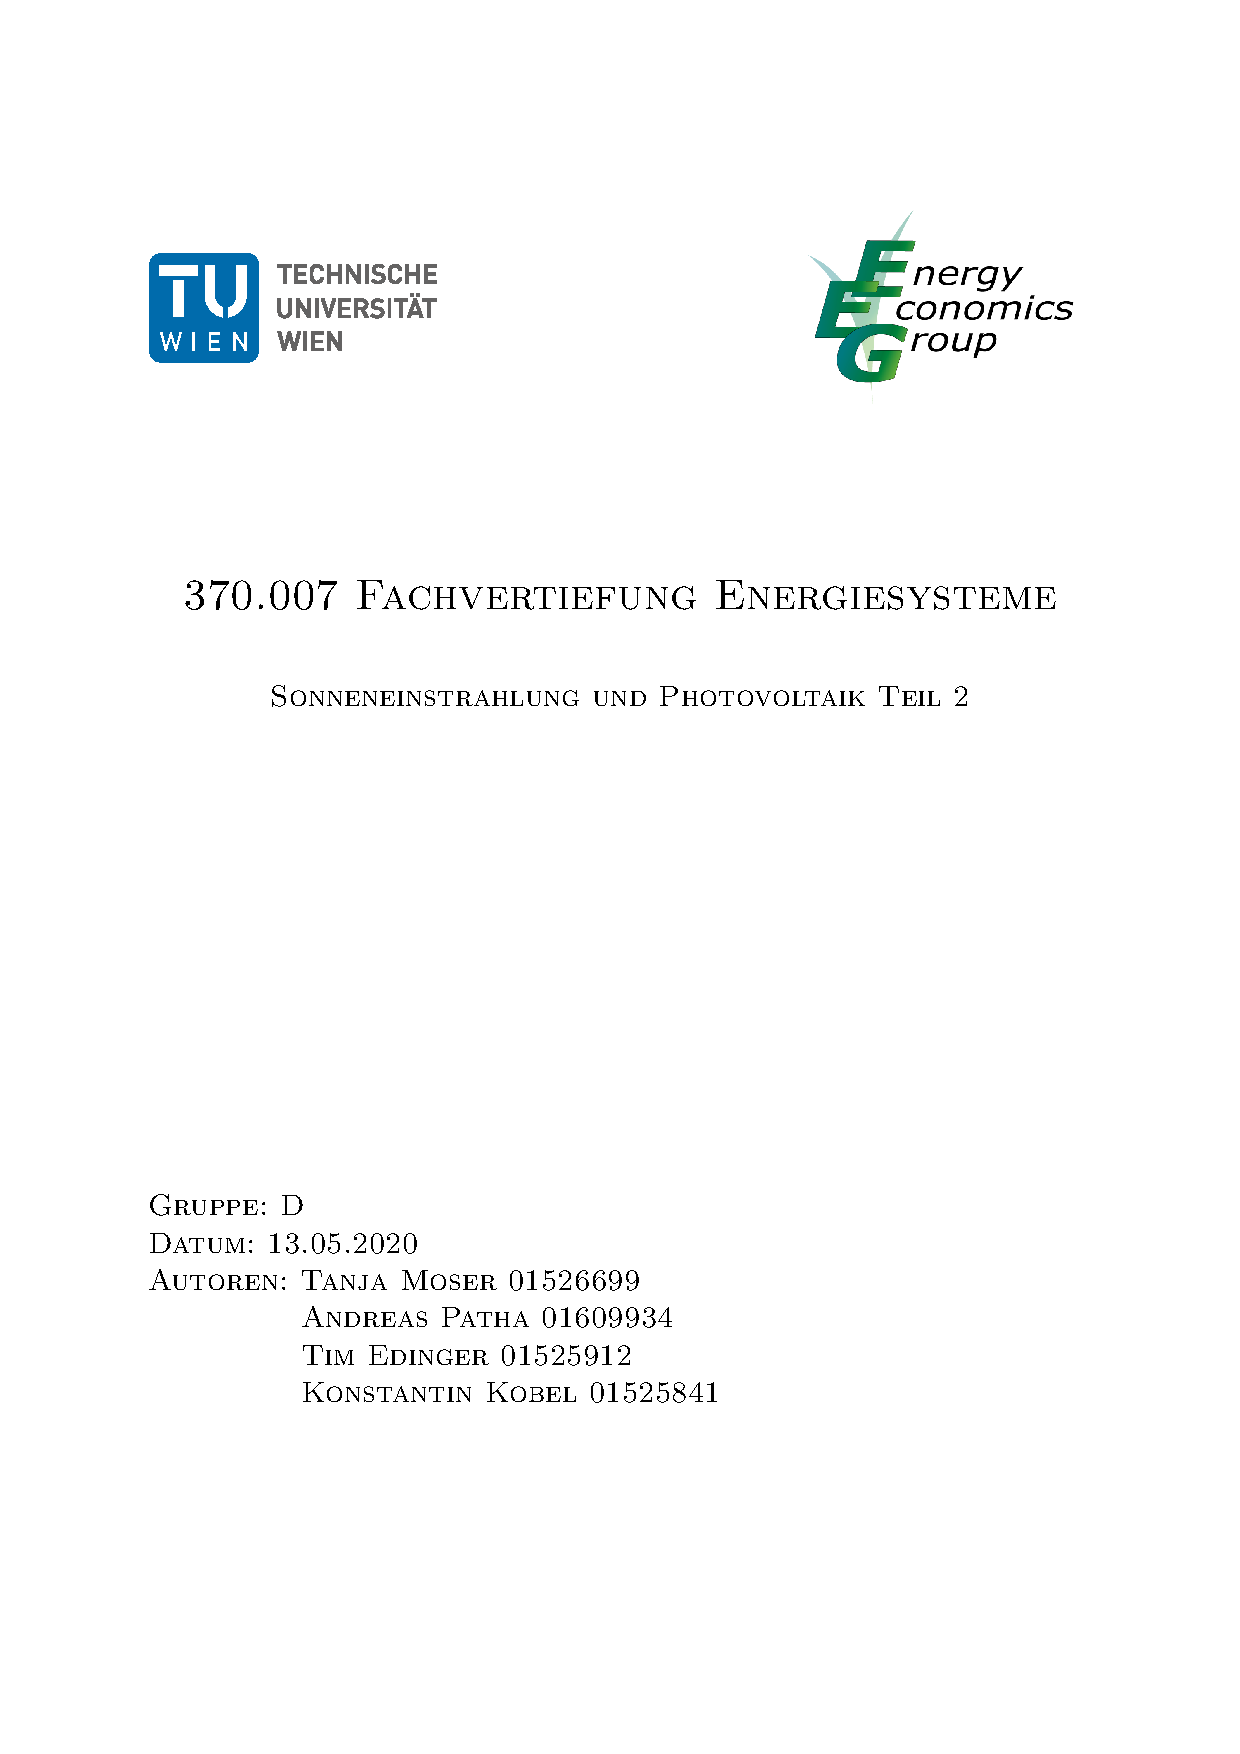
\includepdf{Protokoll_titlepage.pdf}
	
	\newpage
	%Inhaltsverzeichnis
	\tableofcontents
	
	\newpage
	\section{Aufgabenstellung}
	\subsection{Aufgabe 2.1}
	Aufgabe 2.1 befasst sich mit einer PV-Anlage der ersten Übung, unter Einfluss der Temperatur und Einstrahlung mit folgenden Parametern:
	\begin{itemize}
		% Wusste nicht ob ihr die Angaben von dem ersten Protokoll nochmal drin stehen haben wollt!
		%\item Der Standort ist Wien ($48.2^{\circ}$N, $16.3^{\circ}$O).
		%\item Die installierte Leistung ist $1kWp$.
		%\item Der Neigungswinkel der PV-Anlage beträgt $20^{\circ}$.
		%\item Der Azimut der Anlage ist $180^{\circ}$ Süden.
		%\item Die Zeit in Viertelstunden-Werten ist in der Datei $time.mat$ gegeben.\item Anlage am Dach - gut belüftet $c_{T}$ mit dem Wert $0.426$ (für Gelichung 3)
		\item Sonstige Verluste $\eta_{sonst}$ (Reflexion, Temperatur, Wechselrichter, etc.) werden mit dem Wert $0.8$ eingerechnet.				\item Der Modulwirkungsgrad $\eta_{Modul}$ ist $0.17$.
		\item Silizium-Zelle: Koeffizienten $kx, x = 1, ... , 6$ (Huld et al.-Table1 -S.329)
		\item Die Errechnung des Sonnenstandes erfolgt mit der in der Datei $SonnenstandTST.m$ (zur Verfügung gestellten Funktion $SonnenstandTST()$ 	)				\item Die Strahlungsdaten für den Standort sind in der Datei $Strahlung.mat$ gegeben.
		\item Die Daten zur Temperatur sind in der Datei $Temperatur.mat$ gegeben.
	\end{itemize}
	Die Aufgaben lauten:
	\begin{itemize}
		\item[a)] Erweitern Sie das Modell, um die Berücksichtigung des Einflusses der Temperatur und der
Einstrahlung auf den Wirkungsgrad des PV-Moduls (erweitern Sie Ihre Funktion aus
Aufgabe 1.1).
		\item[b)] Vergleichen Sie Ihre Ergebnisse mit jenen aus Aufgabe 1. Wie verändert sich die Verteilung
der Erzeugung über die Jahreszeiten und innerhalb des Tages im Vergleich zum
vereinfachten Ansatz ohne Berücksichtigung von Temperatur- und Strahlungseinfluss auf
den Wirkungsgrad? Stellen Sie dazu die monatlichen Erträge gegenüber sowie die
durchschnittlichen stündlichen Werte.
	\end{itemize}
	\subsection{Aufgabe 2.2}
	Die Unterpunkte der Aufgabe 2.2 lauten:
	\begin{itemize}
		\item[a)] Berechnen Sie die Erzeugung einer 1 kWpeak Anlage (in Wien) unter Abhängigkeit
des Aufstellwinkels (mit Temperatureinfluss). Variieren Sie den Neigungswinkel
der Anlage von $0$ bis $90$ in $2.5$-Intervallen und den Azimut der Anlage von $0$ bis
$360$ in $10$-Schritten.
		\item[b)] Stellen Sie die Volllaststunden der Anlage in Abhängigkeit der Aufstellwinkel in
einer 3D-Grafik dar. Verwenden Sie dazu einmal die Plot-Funktion meshc und
einmal contour, um ISO-Ertragslinien darzustellen.
\begin{itemize}
\item Bei welcher Winkelkombination erhalten Sie den höchsten Ertrag?
\item Zeichnen Sie diesen Punkt in den beiden Darstellungen ein!
\end{itemize}
		\item[c)] Wiederholen Sie die 3D-Berechnung und Darstellung einmal für den Monat Juni
und einmal für Dezember.
\begin{itemize}
\item Was beobachten Sie?
\item Welche Winkelkombinationen würden Sie für die diese beiden Monate empfehlen?
\end{itemize}
	\end{itemize}
	\subsection{Aufgabe 2.3}
	Vergleichen Sie die Erzeugung einer 1 kWpeak Anlage von 2 zusätzlichen (möglichst
unterschiedlichen) Standorten in Europa mit der von Wien. Die Strahlungs- und
Temperaturdaten sind für das Jahr 2005 auf
http://www.soda-pro.com/web-services/radiation/helioclim-3-archives-for-free verfügbar.
	\begin{itemize}
		\item[a)]Vergleichen Sie die Erzeugung der Standorte und zeigen Sie die wesentlichen
Unterschiede zwischen den Standorten:
\begin{itemize}
\item gesamte Jahreserzeugung und Volllaststunden
\item durchschnittliche Tagesproduktion ( 24 Werte pro Standort)
\end{itemize}
	\item[b)] Stellen Sie die Volllaststunden der Anlagen in Abhängigkeit der Aufstellwinkel in
einer Grafik dar. Welche Unterschiede erkennen Sie? Wo liegen jeweils die
optimalen Winkelkombinationen für jeden Standort?
	\item[c)] Beschreiben Sie die Gründe, warum die Erzeugung aus PV-Anlagen an
unterschiedlichen Standorten zeitliche (tageszeitliche und saisonale) Unterschiede
aufweist.
	\end{itemize}
	\newpage
	\section{Berechnungen}
	\subsection{Temperaturabhängigkeit einer PV-Anlage}
	Wie bereits in Kapitel 5 "Interpretation der Ergebnisse" von Protokoll 1 erwähnt, ist der Wirkungsgrad einer PV-Anlage von der Temperatur dieser abhängig. Generell gilt, dass der Wirkungsgrad bei niedrigen Temperaturen steigt und bei hohen Temperaturen sinkt.\newline
	Der temperaturabhängige Wirkungsgrad kann über folgende Formel ermittelt werden:
	\begin{equation}
	\eta_{rel}=1+k_1*\ln{(G')}+k_2*\ln{(G')}^2+T'*(k_3+k_4*\ln{(G')}+k_5*\ln{(G')}^2)+k_6*T'^2
	\end{equation}
	Die Parameter in dieser Gleichung sind folgendermaßen definiert:
	\begin{itemize}
		\item \textbf{$G$} - Dieser Wert entspricht der gesamten, auf die PV-Anlage auftreffenden, Einstrahlung. (Die Berechnung von $G$ wird im ersten Protokoll erklärt.)
		\item \textbf{$T_{mod_{STC}}$} - Dieser Wert wurde als Referenzwert, für die Temperatur des Moduls, in den Standard Test Conditions definiert. Er entspricht $25^{\circ}C$.
		\item \textbf{$G_{STC}$} - Dieser Wert wurde in den Standard Test Conditions als Referenzwert für die einfallende Strahlung definiert. Er entspricht $1000W/m^2$.
		\item \textbf{$c_T$} - Dieser Faktor gibt an, wie stark sich das Modul durch Sonneneinstrahlung erhitzt.
		\item \textbf{$T_{amb}$} - Entspricht der Umgebungstemperatur der PV-Anlage.
		\item \textbf{$T_{mod}$} - Entspricht der tatsächlichen Temperatur des Moduls. Diese errechnet sich zu $T_{amb}+c_T*G$.
		\item \textbf{$G'$} - Dieser Wert ist der Quotient aus der tatsächlichen Einstrahlung $G$ und der in den Standard Test Conditions definierten Einstrahlung $G_{STC}$. Daraus ergibt sich $G'=\frac{G}{G_{STC}}$.
		\item \textbf{$T'$} - Die Temperatur des Moduls wird als Differenz zum Referenzwert $T_{mod_{STC}}$ angegeben. Diese errechnet sich zu $T'=T_{mod}-T_{mod_{STC}}$.
	\end{itemize}
	Die Parameter $k_1$ bis $k_6$, für c-Si Module, müssen durch Messungen gefunden werden. Sie werden im Skript $Mapping the performance of PV modules, effects of module type and data averaging$ folgendermaßen definiert:
	\begin{table}[H]
		\begin{tabular}{|l|c|c|c|c|c|}
			\hline
			\multicolumn{1}{|c|}{$k_1$} & $k_2$     & $k_3$     & $k_4$    & $k_5$    & $k_6$    \\ \hline
			-0.017162                   & -0.040289 & -0.004681 & 0.000148 & 0.000169 & 0.000005 \\ \hline
		\end{tabular}
	\end{table}
	In MATLAB ergibt sich daraus folgender Code:
	\begin{lstlisting}
	Tmod = repelem(Temperatur,4) + ct.*GesGen;
	T = Tmod $-$ TmodSTC;
	TWirkungsgrad=1$-$0.017162*log(GesGen./gSTC)$-$0.040289*log(GesGen./gSTC).^2$-$0.004681.*log(GesGen./gSTC).^3+0.000148.*log(GesGen./gSTC).^4+0.000169.*log(GesGen./gSTC).^5+0.000005.*T.^2;
	\end{lstlisting}
	Da die Temperatur in der Datei $Temperatur.mat$ nur in Stunden-Intervallen gegeben ist, müssen wir den Array der Temperatur dementsprechend skalieren, damit eine Multiplikation mit $GesGen$ möglich ist. ($GesGen$ enthält Viertelstunden-Werte)\newline
	Die Berechnung von $GesGen$ wird im ersten Protokoll erklärt.\newline
	Daraus ergibt sich die temperaturabhängige Energie zu
	\begin{equation}
	E=E_{G,gen}*A*\eta_{Modul}*\eta_{sonst}*\eta_{rel}
	\end{equation}
	Definitionen zu Formel (2) können dem ersten Protokoll entnommen werden.
	\newpage	
	\section{Ergebnisse - Aufgabe 2.1}
	\subsection{1.1.a}
	
	\subsection{1.1.b}

	\section{Ergebnisse - Aufgabe 2.2}
	\subsection{2.2.a}
	
	\subsection{2.2.b}
	
	\subsection{2.2.c}
	
	\section{Ergebnisse - Aufgabe 2.3}
	\subsection{2.3.a}
	
	\subsection{2.3.b}
	
	\subsection{2.3.c}	
	
	\section{Interpretation der Ergebnisse}
	
	\section{Literatur}

\end{document}